% ++++++++++++++++++++++++++++++++++++++++++++++++++++++++++++++++++++++++++++++
% + Document



% ++++++++++++++++++++++++++++++++++++++++++++++++++++++++++++++++++++++++++++++
% + Document class

% ---- Book => 
%\documentclass[11pt]{book}

% ---- Report => front page for title, one side by default
%\documentclass[11pt,twoside,twocolumn,notitlepage]{report}

% ---- Article => no front page for the title by default, no chapters
%\documentclass[11pt,oneside]{article}

%\documentclass[8pt,handout]{beamer} % => handout option flattens the incremental list overlay
\documentclass[8pt]{beamer}

% - end of document class
% ------------------------------------------------------------------------------

%\usetheme{CambridgeUS}

% ++++++++++++++++++++++++++++++++++++++++++++++++++++++++++++++++++++++++++++++
% + Document preamble
% Theme for beamer presentation.
\usepackage{beamerthemesplit} 
% Other themes include: beamerthemesplit, beamerthemebars, beamerthemelined,
%                       beamerthemetree, beamerthemeplain

\beamertemplatenavigationsymbolsempty    % remove navigation bar

\usefonttheme{professionalfonts}

\usepackage{graphicx}
\usepackage{caption}
\usepackage{subcaption}
\usepackage{bm}
\usepackage{epstopdf}

% Add outline frame before each section
%\AtBeginSection[]
%{
%	\begin{frame}{Oultine}
%	\Large{\tableofcontents[currentsection]}
%	\end{frame}
%}

\setbeamerfont{institute}{size=\normalsize}

\newcommand{\squeezeup}{\vspace{-5mm}}

% - end of document preamble
% ------------------------------------------------------------------------------



% ++++++++++++++++++++++++++++++++++++++++++++++++++++++++++++++++++++++++++++++
% + Beginning of content

\begin{document}


\title[CSP group - Imperial College London \hspace{2.4cm}
\insertframenumber/\inserttotalframenumber]
{Sequential local FRI sampling of infinite streams of Diracs}
\author{Jon O\~{n}ativia, Jose Antonio Urig\"{u}en and Pier Luigi Dragotti}
\institute{
Imperial College London\\[0.4cm]
%\includegraphics[scale=0.3]{figures/Imperial_College_London}
ICASSP 2013, Vancouver (Canada)
}
\date{May 30, 2013}      % Enter the date or \today between curly braces


% Creates title page of slide show using above information
\begin{frame}
\titlepage
\end{frame}
\note{Talk for 30 minutes} % Add notes to yourself that will be displayed when typeset with the notes class option.


% ************************
% * Beginning of section

\section*{}
% Creates table of contents slide incorporating all \section and \subsection commands.
\begin{frame}
\frametitle{Outline}
\Large{\tableofcontents}
\end{frame}

% * End of section
% ************************


% ************************
% * Beginning of section

\section[Sampling FRI signals]{Sampling Finite Rate of Innovation Signals}

\subsection{Signals with Finite Rate of Innovation}

%%%%%%%%%%%%%%%%%%%%%%%%%%%%%%%%%%%%%%%%%%%%%%%%%%%%%%%%%%%%%%%%%%%%%%%%%%%%%%%
\begin{frame}
\frametitle{Signals with Finite Rate of Innovation (FRI)}   % Insert frame title between curly braces

\begin{itemize}

\item<1->
Signals that have a finite number of free parameters
\begin{equation*}
x(t) = \sum_{k \in \mathbb{Z}} \; \sum_{r=0}^{R-1} \; a_{k,r} \; g_r(t-t_k).
\end{equation*}
If the set of functions $\lbrace g_r(t) \rbrace_{r=0,1,\ldots,R-1}$ is known, 
the signal $x(t)$ is perfectly determined by the coefficients $(a_{k,r}, t_k)$.
\\[.5cm]

\item<2->
Let us constrain the input signal to a stream of K Diracs in an interval $\tau$
$x(t) = \sum_{k=1}^{K} \; a_k \; \delta(t-t_k)$, where $t_k \in [0,\tau]$.\\
\begin{itemize}
\item<3-> This signal has 2$K$ degrees of freedom in a temporal interval $\tau$
\item<3-> Local rate of innovation: $\rho = \tfrac{2K}{\tau}$
\\[.5cm]
\end{itemize}

\item<4-> We acquire the signal with a sampling device at regular intervals of time $t=nT$

\begin{figure}[h]
\includegraphics[width=.8\linewidth]{figures/samplingDeltaTrain}
\end{figure}

\squeezeup
\item<4-> The output samples can be expressed as 
$y_n = \left\langle x(t), \varphi(t/T - n) \right\rangle$.

\end{itemize}

\end{frame}
%%%%%%%%%%%%%%%%%%%%%%%%%%%%%%%%%%%%%%%%%%%%%%%%%%%%%%%%%%%%%%%%%%%%%%%%%%%%%%%

%%%%%%%%%%%%%%%%%%%%%%%%%%%%%%%%%%%%%%%%%%%%%%%%%%%%%%%%%%%%%%%%%%%%%%%%%%%%%%%
\begin{frame}

\begin{equation*}
x(t) = \sum_{k=1}^{K} \; a_k \; \delta(t-t_k)
\end{equation*}

\begin{itemize}

\item<1-> Classical sampling theory does not allow to sample and perfectly 
reconstruct a stream of Diracs because it is not a bandlimited signal.
\\[.5cm]

\item<2-> The FRI framework can achieve perfect reconstruction under some conditions.
\\[.5cm]

\item<3-> State of the art FRI algoritms do not deal well with infinite streams:
\begin{itemize}
\item Based on isolating bursts of Diracs
\item Require high sampling rates
\\[.5cm]
\end{itemize}

\item<4-> We present a novel sequential algorithm that is able to reconstruct 
these type of signals:
\begin{itemize}
\item Able to recover 1k Diracs from 10k samples
\item Robust under high noise conditions
\item Works in real time
\item Succesfully applied in neuroscience to infere spiking activity of individual 
neurons from calcium fluorescence imaging
\end{itemize}

\end{itemize}

\end{frame}
%%%%%%%%%%%%%%%%%%%%%%%%%%%%%%%%%%%%%%%%%%%%%%%%%%%%%%%%%%%%%%%%%%%%%%%%%%%%%%%


\subsection{Sampling process} 

%%%%%%%%%%%%%%%%%%%%%%%%%%%%%%%%%%%%%%%%%%%%%%%%%%%%%%%%%%%%%%%%%%%%%%%%%%%%%%%
\begin{frame}
\frametitle{Sampling process} 

\begin{itemize}

\item<1-> We sample $x(t)$ with a very specific kernel: $\varphi(t)$ together
with its shifted versions can reproduce exponentials of the form $e^{\alpha_mt}$
\begin{equation*}
\sum_{n \in \mathbb{Z}} c_{m,n} \varphi(t-n) = e^{\alpha_mt}, \quad m = 0, 1, \ldots, P
\end{equation*}

\item<2-> A family of functions that satisfy the exponential reproducing property are the 
exponential splines (E-splines). The Fourier transform of the $P$-th order E-Spline 
with parameter $\vec{\alpha}_P = (\alpha_0, \alpha_1, \ldots, \alpha_P)$ is given by
\begin{equation*}
\hat{\varphi}_{\vec{\alpha}_P}(\omega) 
= 
\prod_{m=0}^P \left( \frac{1-e^{\alpha_m-j\omega}}{j\omega-\alpha_m} \right)
\end{equation*}

\item<3-> If coefficients $\alpha_m$ are real, or complex but appear in complex conjugate
pairs, the kernel is real valued.
\\[.2cm]

\item<3-> E-splines present the advantage of being of compact support $P+1$.

\end{itemize}

\end{frame}
%%%%%%%%%%%%%%%%%%%%%%%%%%%%%%%%%%%%%%%%%%%%%%%%%%%%%%%%%%%%%%%%%%%%%%%%%%%%%%%


%%%%%%%%%%%%%%%%%%%%%%%%%%%%%%%%%%%%%%%%%%%%%%%%%%%%%%%%%%%%%%%%%%%%%%%%%%%%%%%
\begin{frame}

\vspace{.2cm}
\begin{tabular}{ll}
Input signal:                      & $x(t) = \sum_{k=1}^{K} \; a_k \; \delta(t-t_k)$\\[.2cm]
Samples ($T=1)$:                   & $y_n = \left\langle x(t), \varphi(t - n) \right\rangle$\\[.2cm]
$\varphi(t)$ satisfies:            & $\sum_{n \in \mathbb{Z}} c_{m,n} \varphi(t-n) = e^{\alpha_mt}, \quad$
                                     $\alpha_m = \alpha_0 + m \lambda$ and $m=0,\ldots,P$
\end{tabular}
\\[.4cm]

\begin{itemize}

\item<2->
If we combine samples $y_n$ with coefficients $c_{m,n}$ we obtain a new set of 
measurements $s_m$ which can be expressed as a sum of exponentials:
\begin{small}
\begin{equation*}
s_m 
  = \sum_{n} \; c_{m,n} \; y_n
\onslide<3->{
  = \sum_{k=1}^{K} \; \underbrace{a_k \; e^{\alpha_0 t_k}}_{b_k} 
                   \; \left( \underbrace{e^{\lambda t_k}}_{u_k} \right)^m}
\onslide<4->{
  = \sum_{k=1}^{K} \; b_k \; u_k^m}
\end{equation*}
\end{small}

\item<5->
Retrieval of $a_k$ and $t_k$ from samples $s_m$ is a classical problem in spectral
estimation or in direction of arrival (DOA) estimation
\begin{itemize}
\item Can be solved for instance applying the annihilating filter method (a.k.a. Prony's method)
or the matrix pencil method (inspired from ESPRIT)
\\[.4cm]
\end{itemize}

\item<6-> These methods require a minimum number of values $s_m$ and this in turn 
imposes a minimal order $P$ for the sampling kernel: $P+1 \geq 2K$.
\begin{itemize}
\item Critical sampling is achieved for $P+1 = 2K$
\\[.4cm]
\end{itemize}

\item<7-> If we have an infinite stream we face some problems:
\begin{itemize}
\item This approach requires knowledge of all samples $y_n$ in order to compute $s_m$
\item The number of Diracs is infinite so the order of the E-spline must be infinite as well
\end{itemize}

\end{itemize}

\end{frame}
%%%%%%%%%%%%%%%%%%%%%%%%%%%%%%%%%%%%%%%%%%%%%%%%%%%%%%%%%%%%%%%%%%%%%%%%%%%%%%%


\section{Sequential algorithm}

\subsection{Sampling an infinite sequence of Diracs}

%%%%%%%%%%%%%%%%%%%%%%%%%%%%%%%%%%%%%%%%%%%%%%%%%%%%%%%%%%%%%%%%%%%%%%%%%%%%%%%
\begin{frame}
\frametitle{Sampling an infinite sequence of Diracs}

\begin{itemize}

\item We consider a continuous time signal $x(t)$ formed by an infinite stream of Diracs,
$\sum_{k \in \mathbb{Z}} a_k \, \delta \left( t - t_k \right)$.\\[.5cm]

\item<2-> There are an infinite number of Diracs, but with a limited rate
of at most $K$ Diracs per $\tau$ interval.
\begin{figure}[h]
\includegraphics[width=.6\linewidth]{figures/K_diracs_per_tau_interval}
\caption{Infinite stream. Local maximum rate of innovation $\rho = 2K/\tau$ ($K=5$, $\tau=3.125$ s).}
\end{figure}

\end{itemize}

\end{frame}
%%%%%%%%%%%%%%%%%%%%%%%%%%%%%%%%%%%%%%%%%%%%%%%%%%%%%%%%%%%%%%%%%%%%%%%%%%%%%%%

%%%%%%%%%%%%%%%%%%%%%%%%%%%%%%%%%%%%%%%%%%%%%%%%%%%%%%%%%%%%%%%%%%%%%%%%%%%%%%%
\begin{frame}

\begin{itemize}

\item We take advantage of the fact that the sampling kernel is of compact support $(P+1)T$. 
Thus, a Dirac can influence at most $P+1$ samples $y_n$.
\\[.2cm]

\item<2-> The sequential algorithm estimates the locations of the Diracs within a sliding
window that covers the interval of time $\tau = NT$.
\\[.2cm]

\begin{figure}[h]
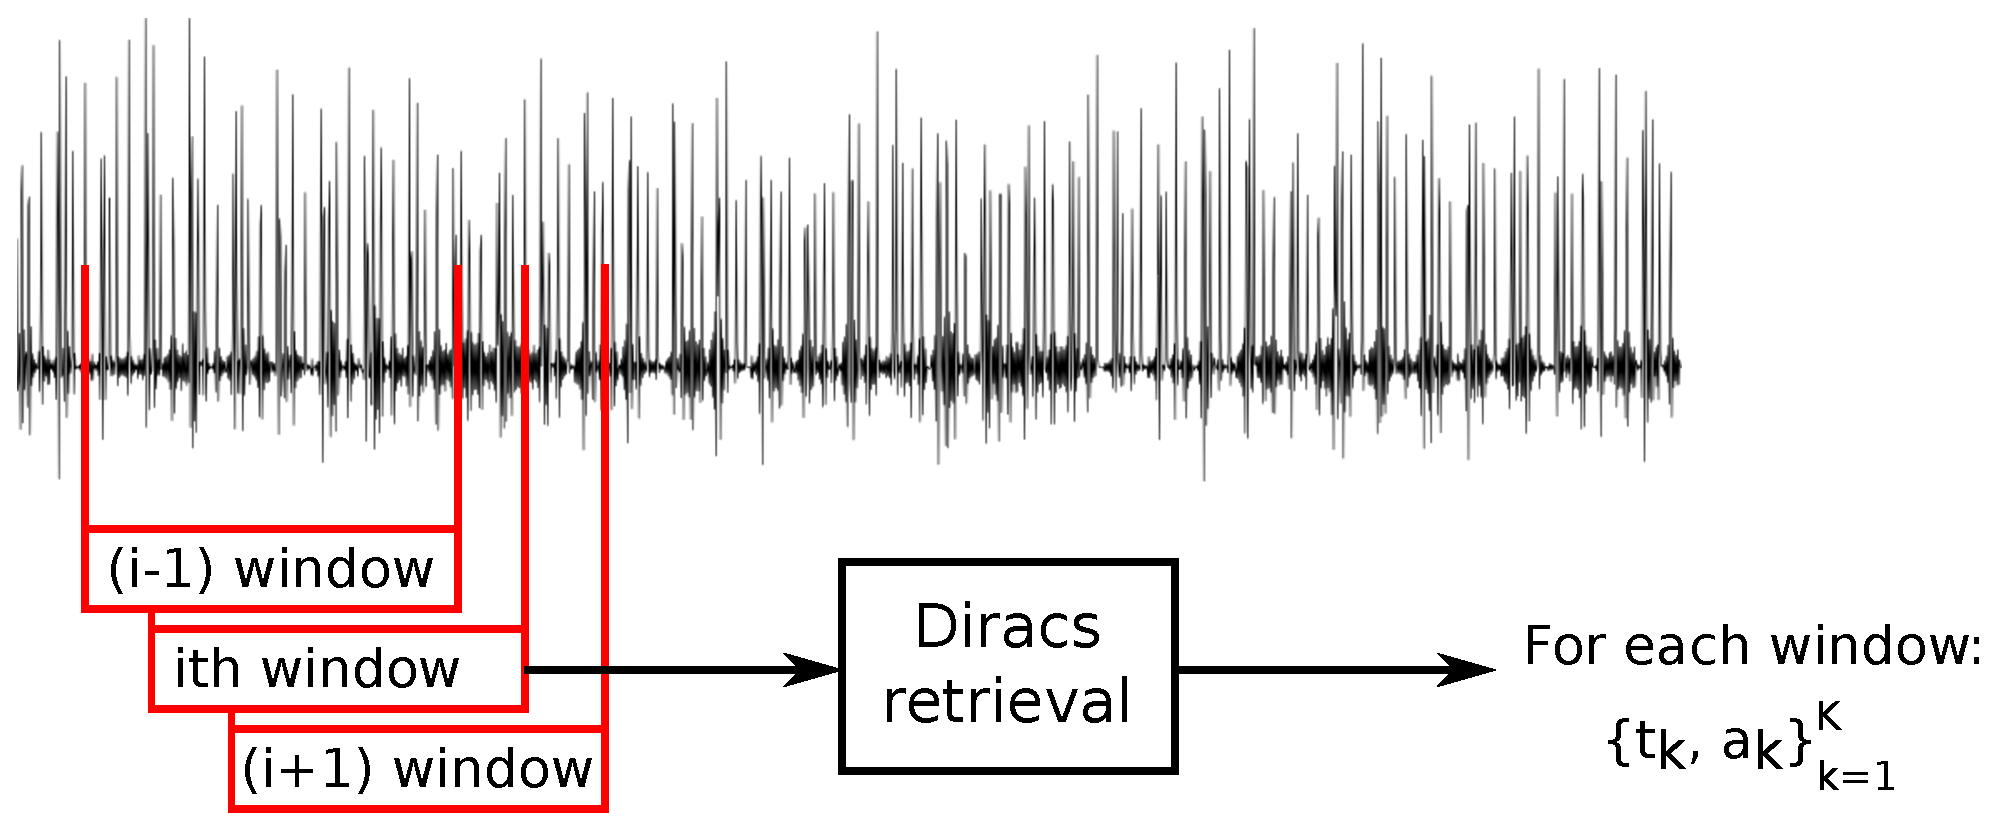
\includegraphics[width=.6\linewidth]{figures/sliding_window}
\caption{Sequential processing.}
\end{figure}

\item<3-> Problem $\Rightarrow$ if we only process $N$ samples at a time there are border 
effects when Diracs are located near the borders of the sliding window
\begin{figure}[h]
\begin{subfigure}{.25\textwidth}
\includegraphics[width=\linewidth]{figures/border_effect_left}
\end{subfigure}
\begin{subfigure}{.25\textwidth}
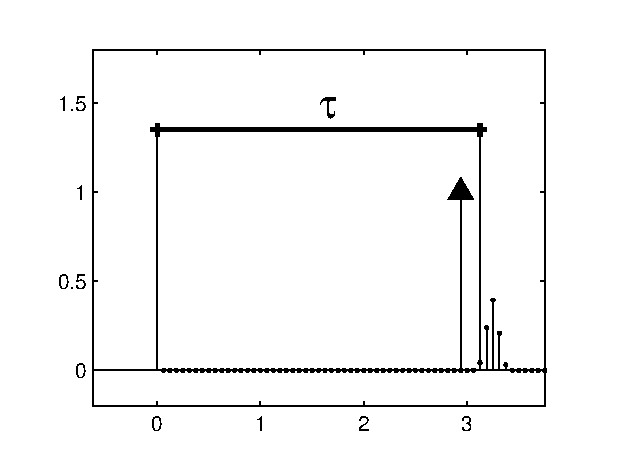
\includegraphics[width=\linewidth]{figures/border_effect_right}
\end{subfigure}
\caption{Border effects.}
\end{figure}

\end{itemize}

\end{frame}
%%%%%%%%%%%%%%%%%%%%%%%%%%%%%%%%%%%%%%%%%%%%%%%%%%%%%%%%%%%%%%%%%%%%%%%%%%%%%%%

%%%%%%%%%%%%%%%%%%%%%%%%%%%%%%%%%%%%%%%%%%%%%%%%%%%%%%%%%%%%%%%%%%%%%%%%%%%%%%%
\begin{frame}

\begin{itemize}

\item The border effect in the left side is due to Dircas before the $\tau$ interval
that leak into the $N$ samples $y_n$ of the current window.

\item<2-> If we assume that we have already recovered Diracs up to the current position of
the sliding window we can remove the contribution to $y_n$ of nearby Diracs that happened before.

\end{itemize}

\only<1>{
\begin{figure}[h]
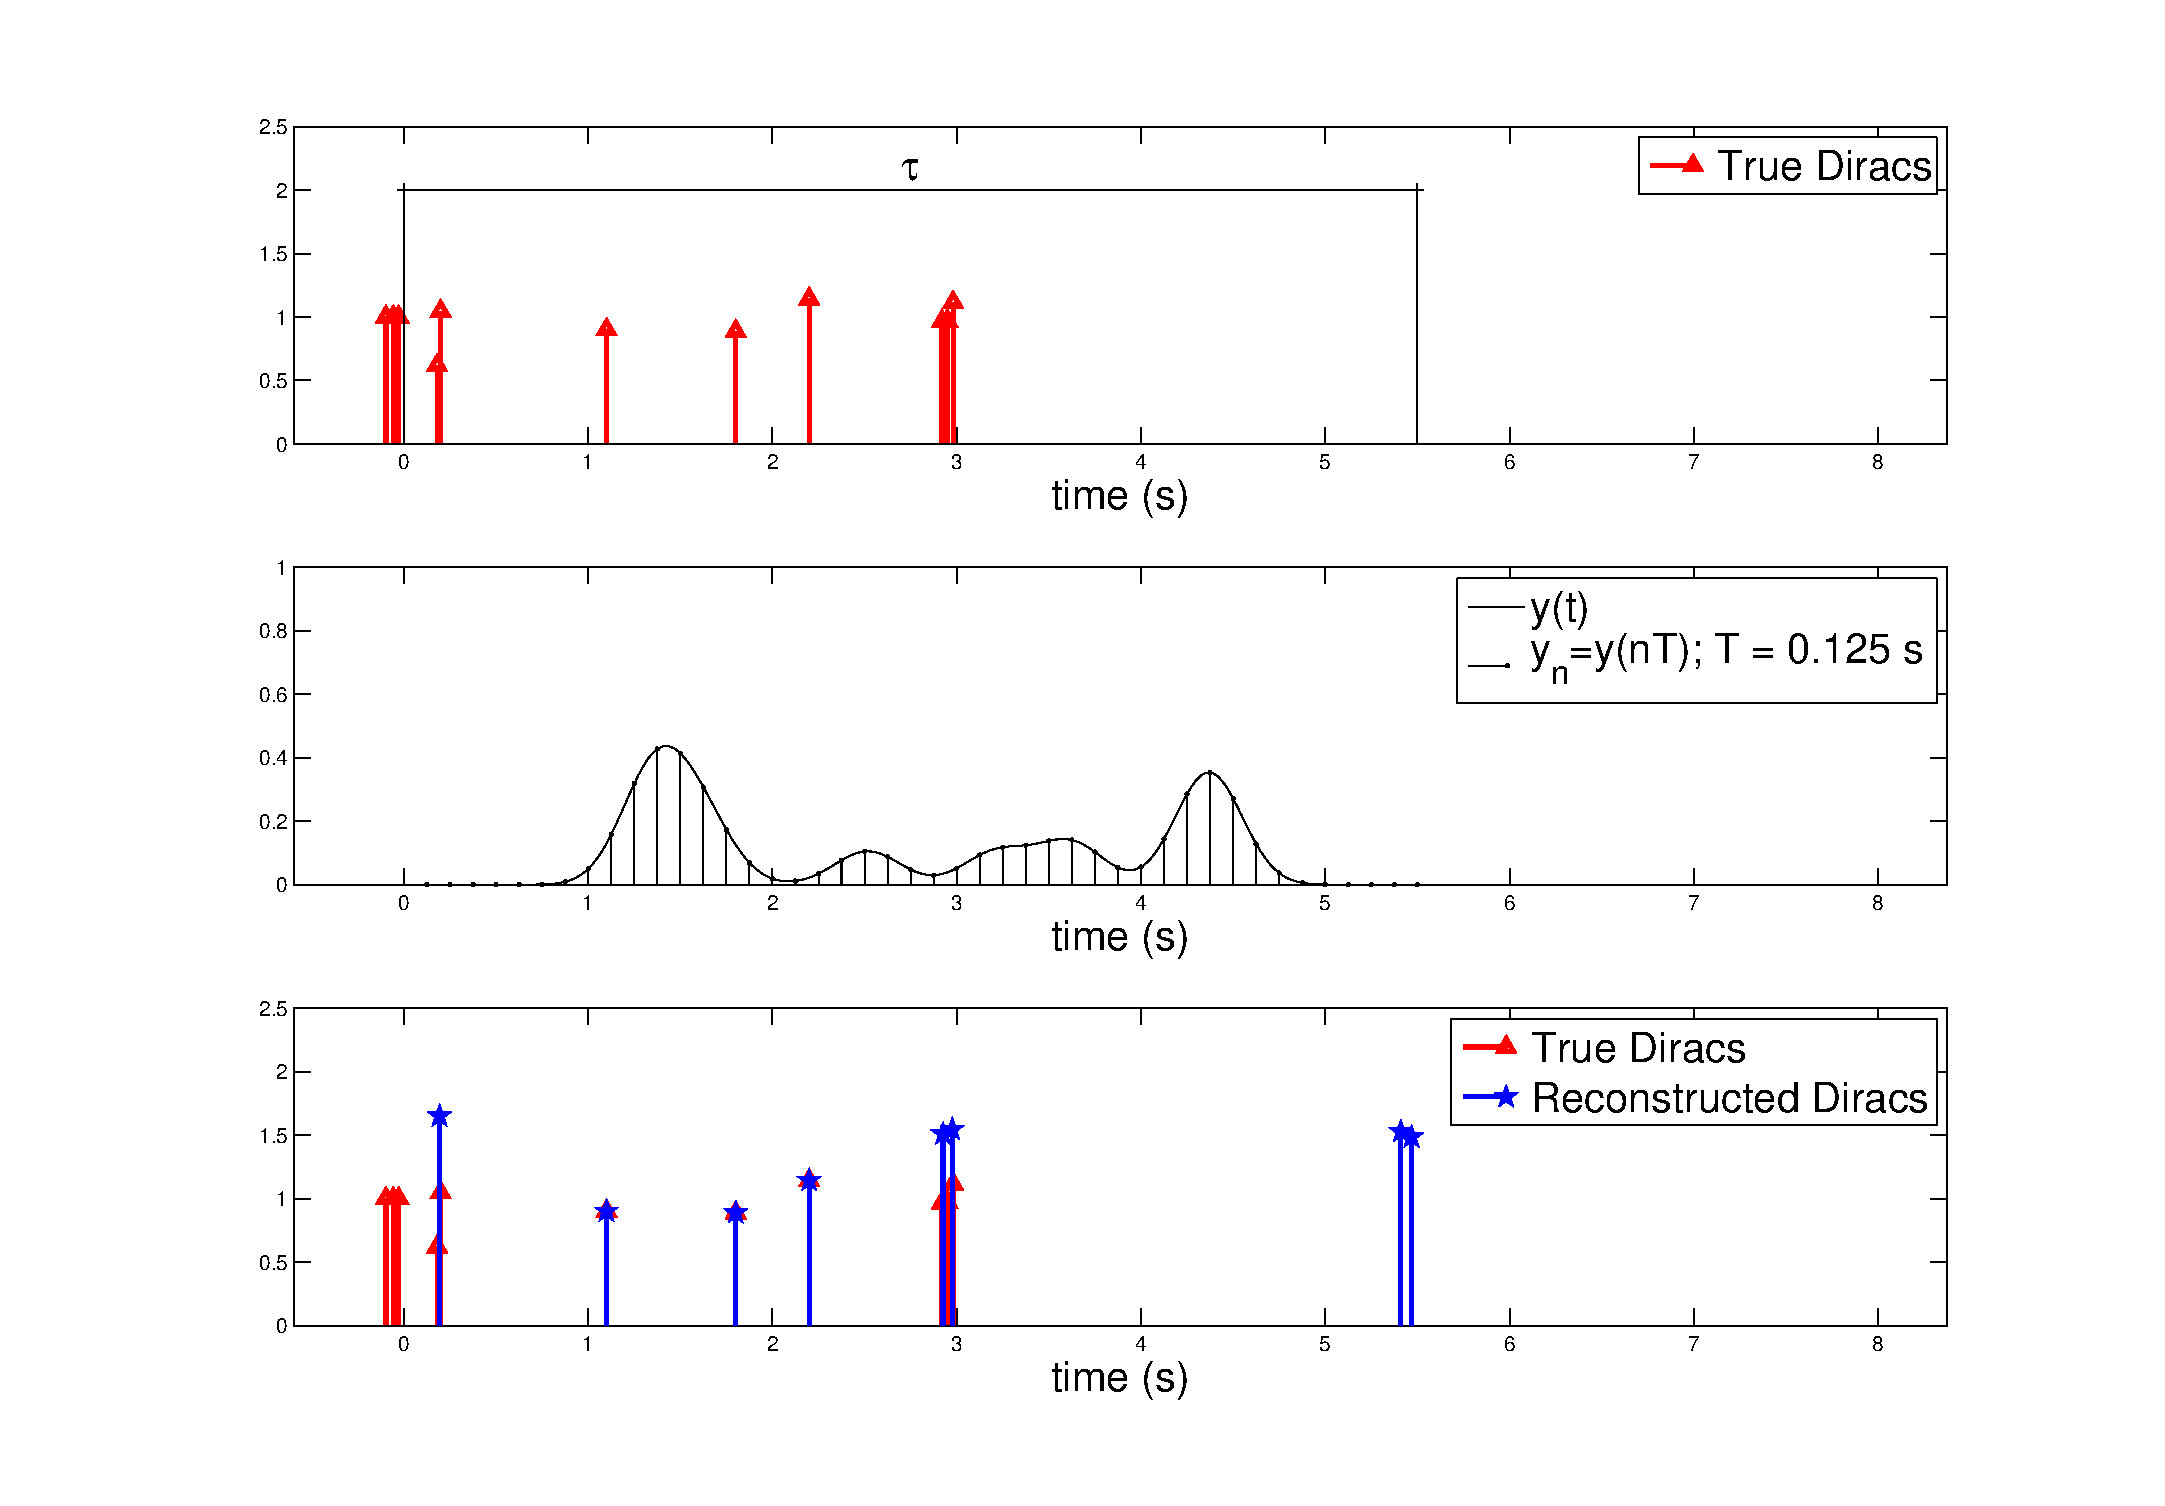
\includegraphics[width=.8\linewidth]{figures/border_remove_1}
\caption{Diracs are not perfectly recovered because past Diracs corrupt current samples.}
\end{figure}
}
\only<2>{
\begin{figure}[h]
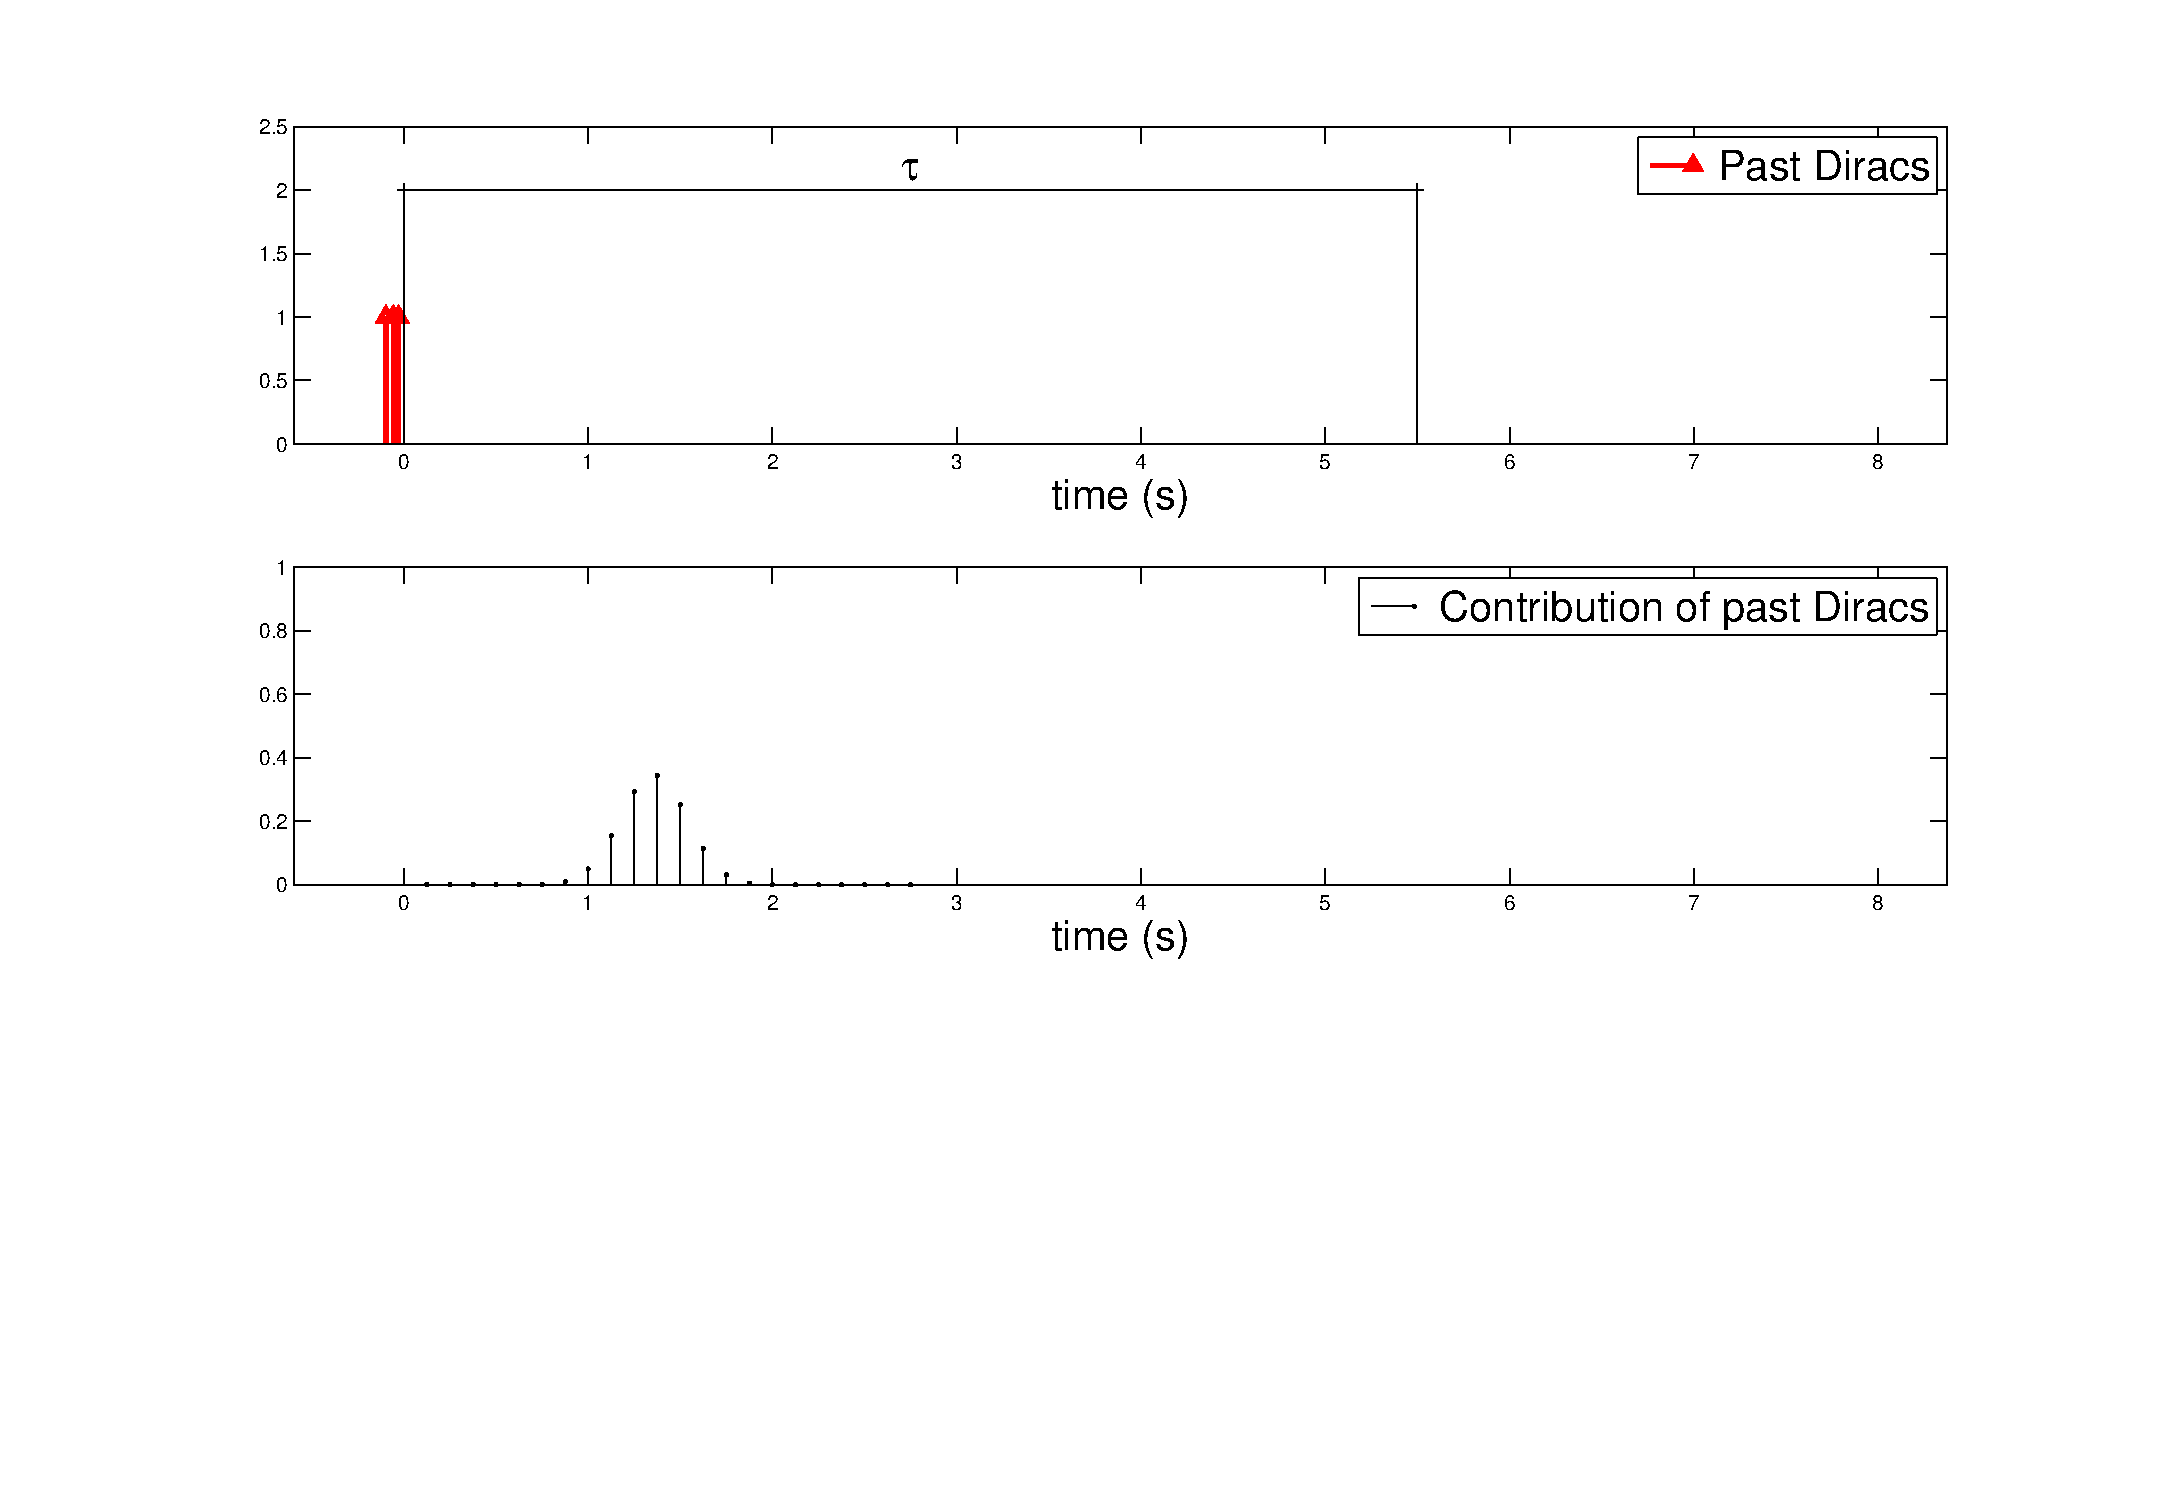
\includegraphics[width=.8\linewidth]{figures/border_remove_2}
\caption{Contribution of past Diracs to samples $y_n$.}
\end{figure}
}
\only<3>{
\begin{figure}[h]
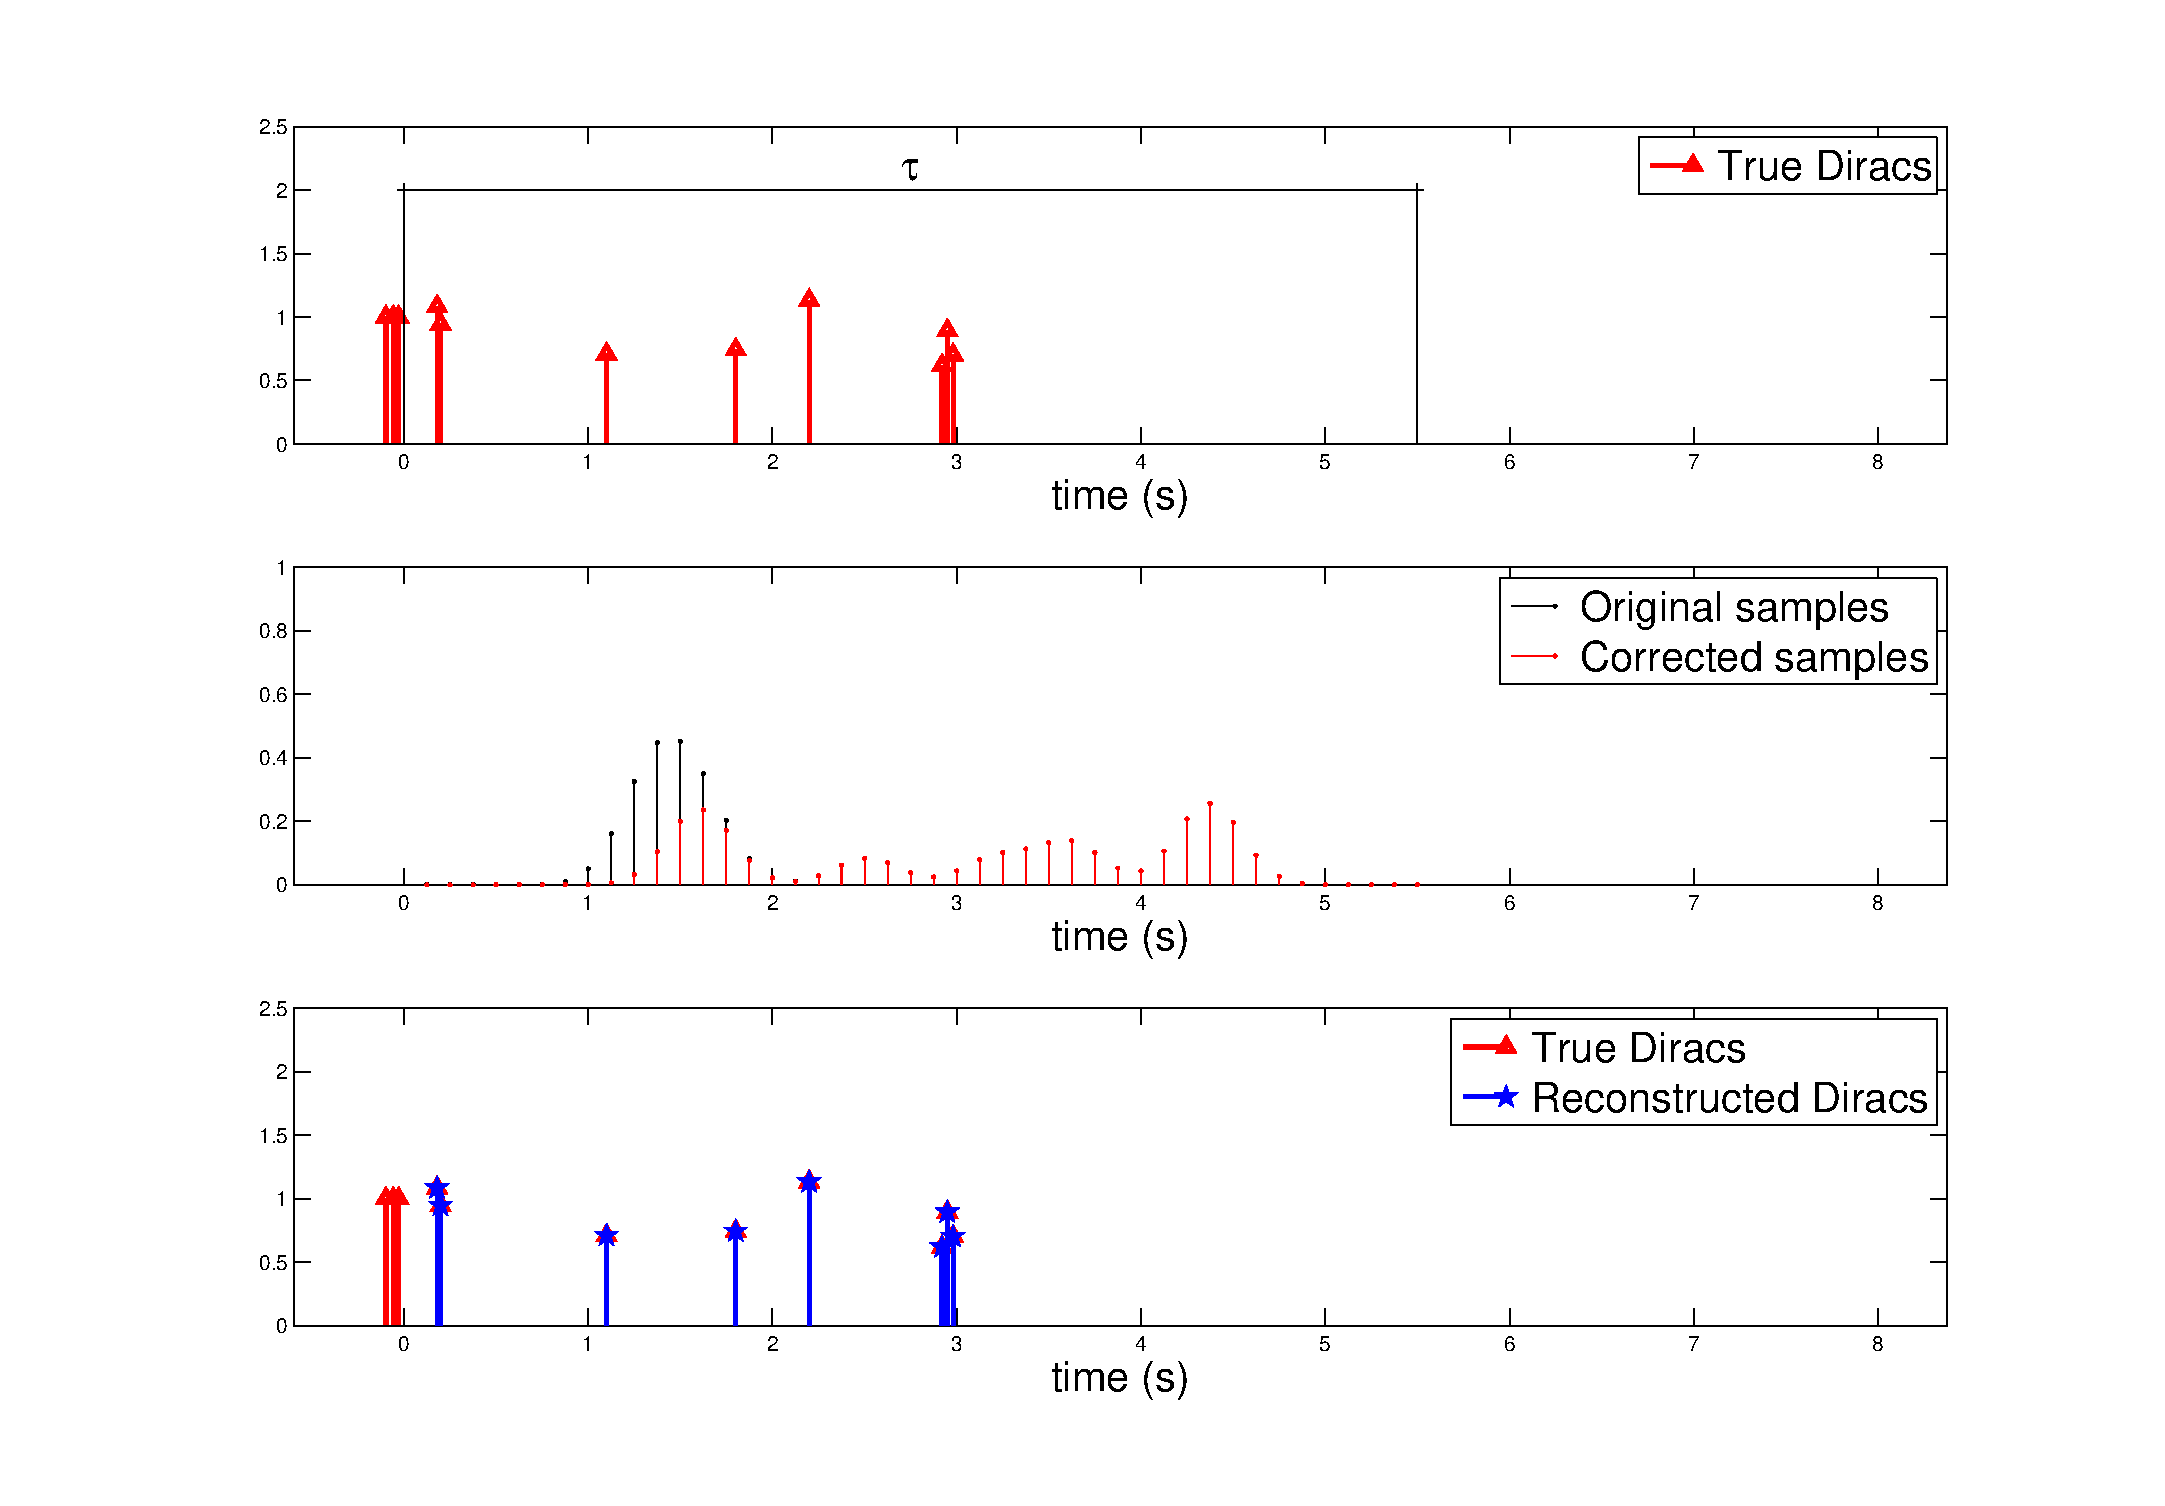
\includegraphics[width=.8\linewidth]{figures/border_remove_3}
\caption{Perfect reconstruction after correcting past Diracs effect.}
\end{figure}
}

\end{frame}
%%%%%%%%%%%%%%%%%%%%%%%%%%%%%%%%%%%%%%%%%%%%%%%%%%%%%%%%%%%%%%%%%%%%%%%%%%%%%%%


%%%%%%%%%%%%%%%%%%%%%%%%%%%%%%%%%%%%%%%%%%%%%%%%%%%%%%%%%%%%%%%%%%%%%%%%%%%%%%%
\begin{frame}

\begin{itemize}

\item The border effect on the right side is due to Diracs inside the $\tau$ interval
that leak outside the $N$ samples $y_n$ of the current window.
\\[.2cm]

\item<2-> To make sure that these Diracs will be recovered for a certain position of 
the sliding window we have to impose:
\begin{equation*}
\boxed{T \leq \tfrac{1}{K\,\rho}} \qquad \text{and} \qquad \boxed{P+1 = 2K}
\end{equation*}

\end{itemize}

\uncover<3->{
\begin{figure}[h]
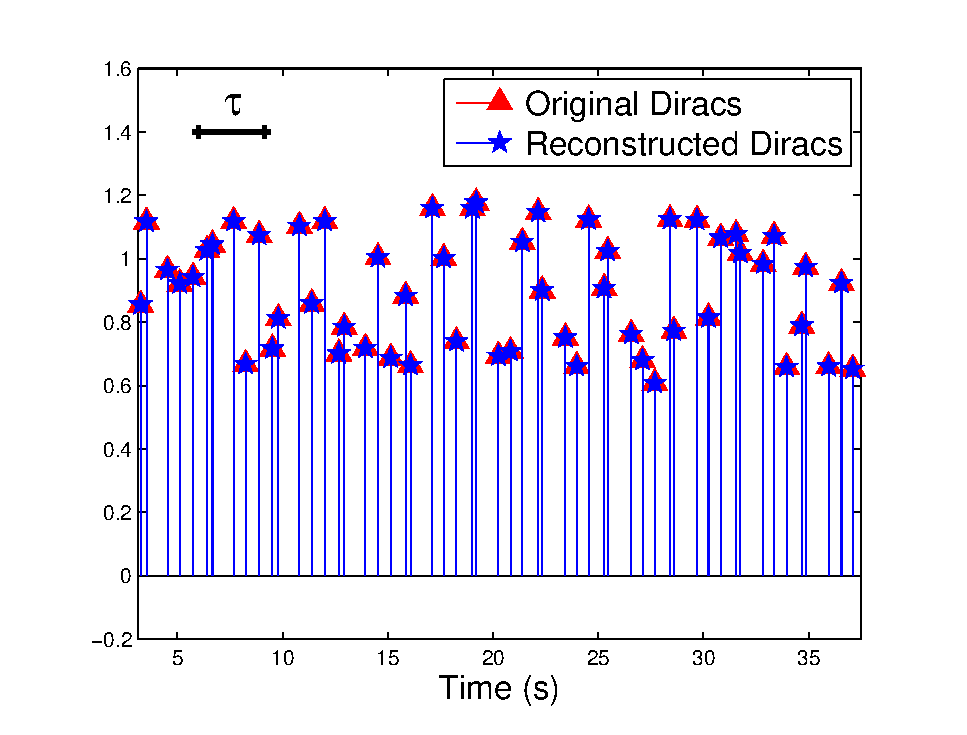
\includegraphics[width=.5\linewidth]{figures/diracs_perf_reconstr}
\caption{Sequential perfect reconstruction of a noiseless stream of Diracs.
Section of a stream of $1000$ Diracs and $10220$ samples $y_n$.
Rate $K=5$ Diracs per $\tau=3.125$ s, $N=50$ samples, $T=1/16$ s and order of the E-spline $P=9$.}
\end{figure}
}

\end{frame}
%%%%%%%%%%%%%%%%%%%%%%%%%%%%%%%%%%%%%%%%%%%%%%%%%%%%%%%%%%%%%%%%%%%%%%%%%%%%%%%


\subsection{The noisy scenario}

%%%%%%%%%%%%%%%%%%%%%%%%%%%%%%%%%%%%%%%%%%%%%%%%%%%%%%%%%%%%%%%%%%%%%%%%%%%%%%%
\begin{frame}
\frametitle{The noisy scenario}

\begin{figure}[h]
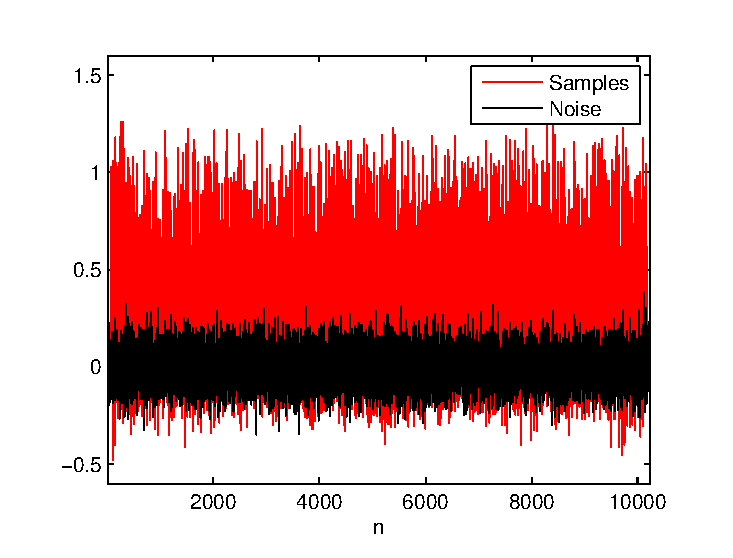
\includegraphics[width=.4\linewidth]{figures/noisy_samples}
\caption{1k Diracs, 10k samples, SNR = 10 dB.}
\end{figure}

\begin{itemize}
\item Perfect reconstruction conditions do not hold anymore.

\item We can relax conditions on $T$ and $P$ 
\begin{itemize}
\item We allow the sampling kernel to be of higher order in order to be more robust against noise.
\end{itemize}

\item The idea is to estimate Diracs by analysing the consistency of the retrieved 
locations among different positions of the sliding window.

\end{itemize}

\end{frame}
%%%%%%%%%%%%%%%%%%%%%%%%%%%%%%%%%%%%%%%%%%%%%%%%%%%%%%%%%%%%%%%%%%%%%%%%%%%%%%%

%%%%%%%%%%%%%%%%%%%%%%%%%%%%%%%%%%%%%%%%%%%%%%%%%%%%%%%%%%%%%%%%%%%%%%%%%%%%%%%
\begin{frame}

\begin{itemize}

\item<1-> A Dirac is captured among different positions of the sliding window:
\begin{itemize}
\item If a retrieved location corresponds to a true Dirac this location will be consistent among 
different positions of the sliding window.
\end{itemize}

\only<1>{
\begin{figure}[h]
\includegraphics[width=.8\linewidth]{figures/sequential_processing_1}
%\caption{Sequential processing of infinite stream.}
\end{figure}
}
\only<2>{
\begin{figure}[h]
\includegraphics[width=.8\linewidth]{figures/sequential_processing_2}
%\caption{Sequential processing of infinite stream.}
\end{figure}
}
\only<3>{
\begin{figure}[h]
\includegraphics[width=.8\linewidth]{figures/sequential_processing_3}
%\caption{Sequential processing of infinite stream.}
\end{figure}
}
\only<4>{
\begin{figure}[h]
\includegraphics[width=.8\linewidth]{figures/sequential_processing_4}
%\caption{Sequential processing of infinite stream.}
\end{figure}
}
\only<5>{
\begin{figure}[h]
\includegraphics[width=.8\linewidth]{figures/sequential_processing_5}
%\caption{Sequential processing of infinite stream.}
\end{figure}
}
\only<6>{
\begin{figure}[h]
\includegraphics[width=.8\linewidth]{figures/sequential_processing_6}
%\caption{Sequential processing of infinite stream.}
\end{figure}
}
\only<7->{
\begin{figure}[h]
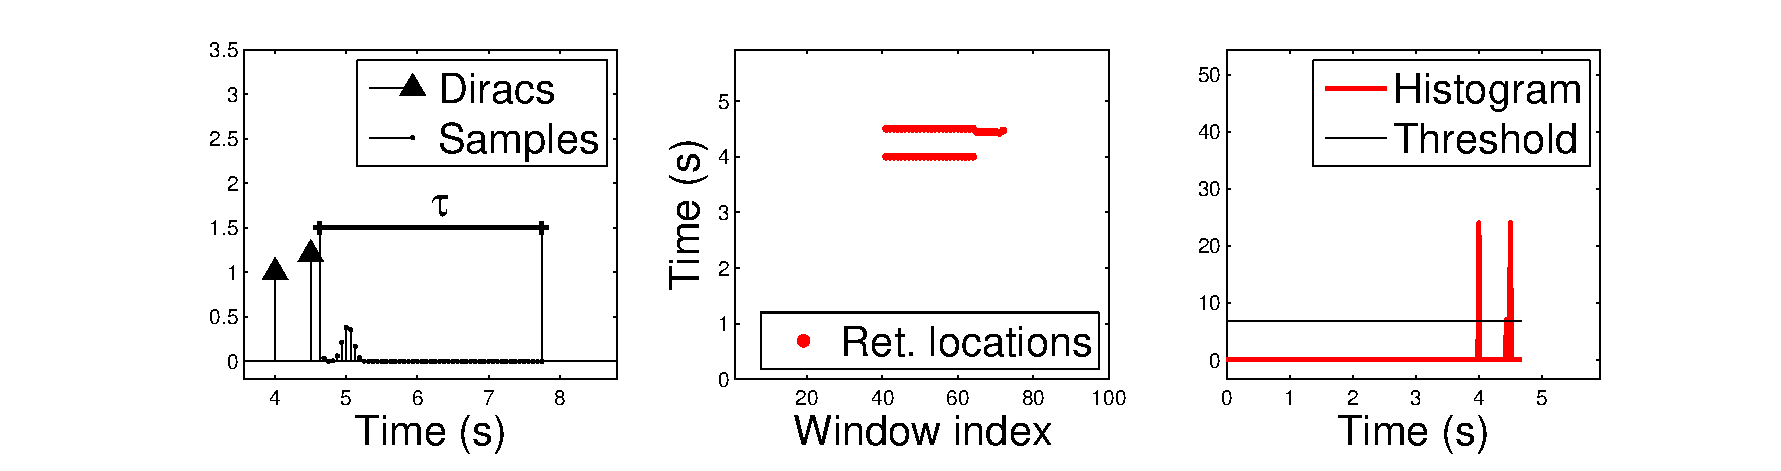
\includegraphics[width=.8\linewidth]{figures/sequential_processing_7}
%\caption{Sequential processing of infinite stream.}
\end{figure}
}

\item<8-> If we analyse the consistency of the retrieved locations we can estimate 
the Diracs from the peaks of the histogram of the locations:

\begin{figure}[h]
\begin{subfigure}{.3\textwidth}
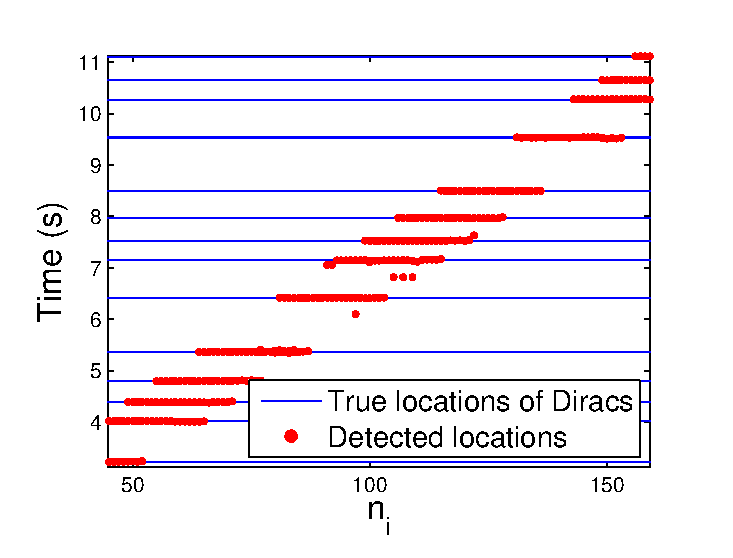
\includegraphics[width=\linewidth]{figures/noisy_scatter}
\end{subfigure}
\begin{subfigure}{.3\textwidth}
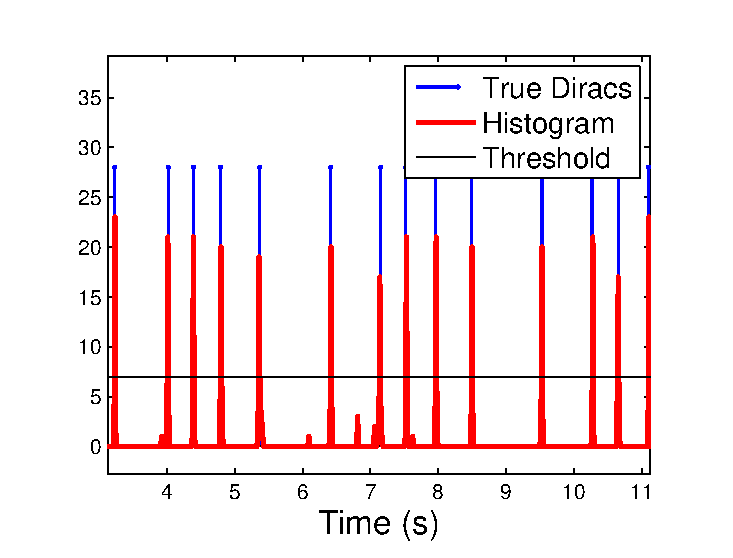
\includegraphics[width=\linewidth]{figures/noisy_histogram}
\end{subfigure}
\caption{Retrieved locations among different positions of the sliding window and histogram
of locations.}
\end{figure}

\end{itemize}

\end{frame}
%%%%%%%%%%%%%%%%%%%%%%%%%%%%%%%%%%%%%%%%%%%%%%%%%%%%%%%%%%%%%%%%%%%%%%%%%%%%%%%

%%%%%%%%%%%%%%%%%%%%%%%%%%%%%%%%%%%%%%%%%%%%%%%%%%%%%%%%%%%%%%%%%%%%%%%%%%%%%%%
\begin{frame}

\begin{itemize}

\item<1-> The consistency analysis makes the retrieval algorithm robust against noise.

\begin{figure}[h]
\begin{subfigure}{.3\textwidth}
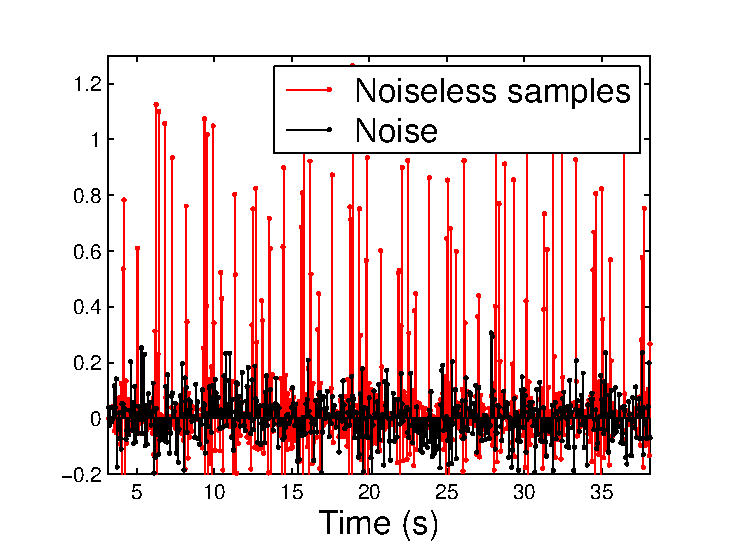
\includegraphics[width=\linewidth]{figures/noisy_samples2}
\end{subfigure}
\begin{subfigure}{.3\textwidth}
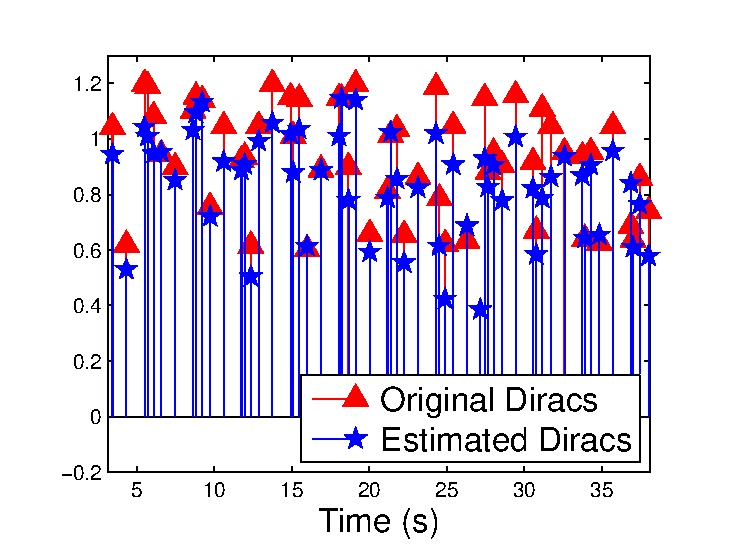
\includegraphics[width=\linewidth]{figures/noisy_diracs_reconstr}
\end{subfigure}
\caption{Sequential reconstruction of a noisy stream of Diracs (SNR = 10 dB).
Section of a stream of $1000$ Diracs and $10220$ samples $y_n$.
Rate $K=5$ Diracs per $\tau=3.125$ s, $N=50$ samples, $T=1/16$ s and order of the E-spline $P=22$.}
\end{figure}

\item<2-> Some results for differents levels of noise (experiment repeated 100 times 
for each level of noise):\\[.2cm]

\begin{center}
\begin{tabular}{|l|c|c|c|c|}
\hline 
SNR (dB)                     & 5         & 10        & 15        &   20      \\
\hline
\hline
Detection rate               & 97.69 \%  & 99.97 \%  & 100.00 \% & 100.00 \% \\
\hline
False positives              & 351.7     & 37.8      & 0.5       & 0.3       \\
\hline
Precision (s)                & 0.0086    & 0.0049    & 0.0028    & 0.0018    \\
\hline
\end{tabular}
\end{center}

\end{itemize}

\end{frame}
%%%%%%%%%%%%%%%%%%%%%%%%%%%%%%%%%%%%%%%%%%%%%%%%%%%%%%%%%%%%%%%%%%%%%%%%%%%%%%%

\subsection{Application: neural activity detection}

%%%%%%%%%%%%%%%%%%%%%%%%%%%%%%%%%%%%%%%%%%%%%%%%%%%%%%%%%%%%%%%%%%%%%%%%%%%%%%%
\begin{frame}
\frametitle{Application: neural activity detection}

\begin{itemize}

\item<1-> This framework has been successfully applied to the detection of neural activity in 
calcium concentration movies
\footnote{Jon O\~{n}ativia, Simon R. Schultz and Pier Luigi Dragotti. 
\textit{A finite rate of innovation algorithm for fast and accurate spike detection from
two-photon calcium imaging.} to appear in Journal of Neural Engineering}.


\begin{figure}[h]
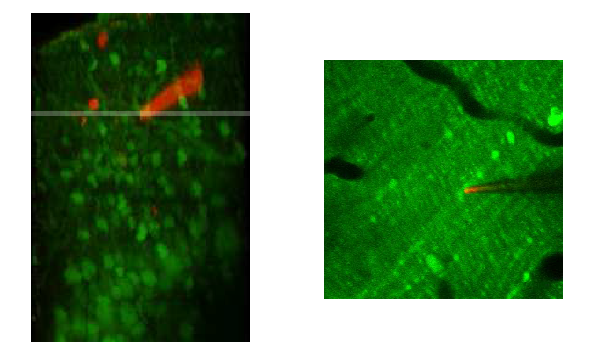
\includegraphics[width=.3\linewidth]{figures/calcium}
\caption{Simultaneous multiphoton calcium imaging of a region of the cortex 
and electrophisiological recording of a targeted cell with a micropipette.}
\end{figure}

\item<2-> Fluorescence sequences obtained by averaging the pixel values of a ROI
can be modeled as a stream of decaying exponentials:

\begin{tiny}
\begin{equation*}
c(t) 
= A \, \sum_{k} e^{-\alpha(t-t_k)} \, u(t-t_k)
\onslide<3->{
= \underbrace{\sum_{k} \delta(t-t_k)}_{x(t)} \; * \;
  \underbrace{A \, e^{-\alpha t} \, u(t)}_{\rho_\alpha(t)}}
\onslide<4->{
= x(t) * \rho_\alpha(t).}
\end{equation*}
\end{tiny}

\item<5-> This is a Finite Rate of Innovation signal and with a correct processing 
of the fluorescence samples we can apply our sequential algorithm.

\end{itemize}

\end{frame}
%%%%%%%%%%%%%%%%%%%%%%%%%%%%%%%%%%%%%%%%%%%%%%%%%%%%%%%%%%%%%%%%%%%%%%%%%%%%%%%


%%%%%%%%%%%%%%%%%%%%%%%%%%%%%%%%%%%%%%%%%%%%%%%%%%%%%%%%%%%%%%%%%%%%%%%%%%%%%%%
\begin{frame}


\begin{itemize}

\item<1-> We achieve 84 \% detection rates with real data (calcium fluorescence sequence)
for electrophysiologically confirmed action potentials.\\[.3cm]

\item<2-> We outperform state of the art real time spike train inference algorithms:

\begin{figure}[h]
\begin{subfigure}{.55\textwidth}
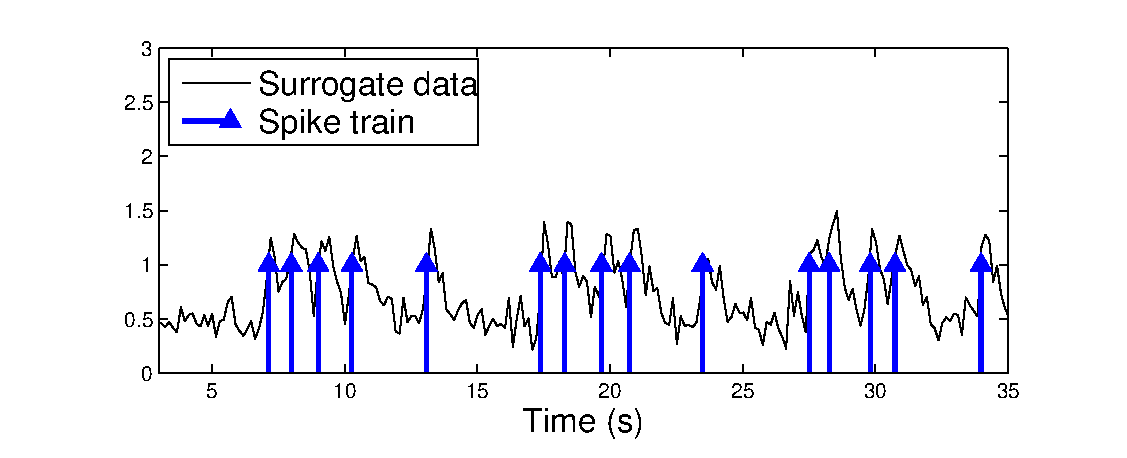
\includegraphics[width=\linewidth]{figures/surrogate_data}
\end{subfigure}
\begin{subfigure}{.35\textwidth}
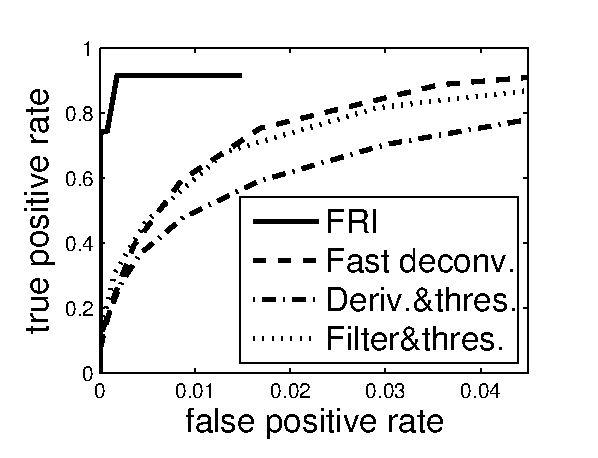
\includegraphics[width=\linewidth]{figures/surrogate_roc_10dB}
\end{subfigure}
\caption{Receiver operating characteristic (ROC) curves for various algorithms with
surrogate data (SNR = 10 dB).}
\end{figure}

\item<3-> This technique can be used to monitor tens of neurons simultaneously since the fluorsecence 
movie captures a volume that contains many neurons.\\[.3cm]

\item<4-> The algorithm is fast enough to perform real-time spike inference:
\begin{itemize}
\item The current MATLAB implementation can process more than 80 datastreams in parallel on a commercial 
laptop (2.5 GHz Intel Core i5 CPU).
\end{itemize}

\end{itemize}

\end{frame}
%%%%%%%%%%%%%%%%%%%%%%%%%%%%%%%%%%%%%%%%%%%%%%%%%%%%%%%%%%%%%%%%%%%%%%%%%%%%%%%

\section*{}

%%%%%%%%%%%%%%%%%%%%%%%%%%%%%%%%%%%%%%%%%%%%%%%%%%%%%%%%%%%%%%%%%%%%%%%%%%%%%%%
\begin{frame}
\begin{center}
\centering{
\Huge{Questions?}
}
\end{center}
\end{frame}
%%%%%%%%%%%%%%%%%%%%%%%%%%%%%%%%%%%%%%%%%%%%%%%%%%%%%%%%%%%%%%%%%%%%%%%%%%%%%%%


\end{document}

% - end of content
% ------------------------------------------------------------------------------



% - end of document
% ------------------------------------------------------------------------------


